\subsection{YugaByteDB}

YugaByteDB merupakan basis data relasional terdistribusi dengan konsensus Raft. YugaByteDB memenuhi prinsip ACID dan terdistribusi secara \textit{native}. YugaByteDB \textit{compatible} dengan API Cassandra (YCQL) dan API Postgres (YSQL).

YugaByteDB memanfaatkan \textit{sharding} untuk mencapai \textit{high availability} dan toleransi kegagalan. Tablet yang berisi grup data direplikasi pada beberapa \textit{instance}. Dengan begitu, penulisan dapat dilakukan pada \textit{instance} yang berbeda dan operasi pembacaan dapat dilakukan pada banyak \textit{instance} \parencite{yugabyteBaeldung}.

\begin{figure}[htbp]
    \centering
    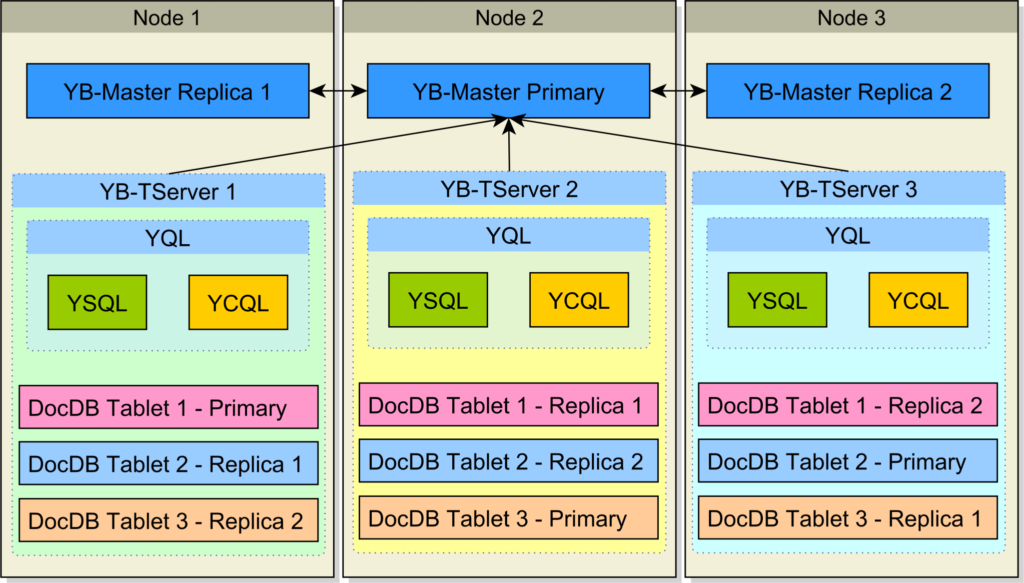
\includegraphics[width=1\textwidth]{resources/chapter-2/yugabyte.png}
    \caption{Arsitektur YugaByteDB \parencite{yugabyteBaeldung}}
    \label{fig:yugabyte-architecture}
\end{figure}

YugaByteDB terdiri atas Master dan TServer. Master merupakan layer kontrol yang mengatur operasi pada kluster dan metadata. TServer bertugas untuk menyimpan dan mengatur data yang disimpan.
